% This appendix is input by manuscript.tex after the references.
\providecommand{\method}{RoadOcc}
\providecommand{\metricup}{\ensuremath{\uparrow}}
\providecommand{\metricdown}{\ensuremath{\downarrow}}
\graphicspath{{supplementary/}{./supplementary/}{./}}
\setcounter{figure}{0}
\setcounter{table}{0}
\renewcommand{\thefigure}{A\arabic{figure}}
\renewcommand{\thetable}{A\arabic{table}}

\newcolumntype{C}[1]{>{\centering\arraybackslash}m{#1}}
\newcolumntype{L}[1]{>{\raggedright\arraybackslash}m{#1}}


\section{Overview}
This supplement documents the implementation and controlled evidence underlying
\method{}. (1) Sections~\ref{sec:sensor_setup}--\ref{sec:velocity_target_contract}
define the fixed-roadside data and velocity targets used to construct historical
addresses. (2) Section~\ref{sec:metrics} specifies the coupled occupancy,
motion, and coverage diagnostics used to assess those addresses and their routed
sources. (3) Sections~\ref{sec:training_objectives}--\ref{sec:exact_contract}
provide the scale-wise objectives and exact DCA--VVE--VDSF execution contract.
(4) Sections~\ref{sec:model_size}--\ref{sec:visuals} report efficiency,
controlled studies, and scope under the complete model configuration.

\section{Roadside Sensor Configuration}
\label{sec:sensor_setup}

\begin{wrapfigure}{r}{0.50\columnwidth}
  \centering
  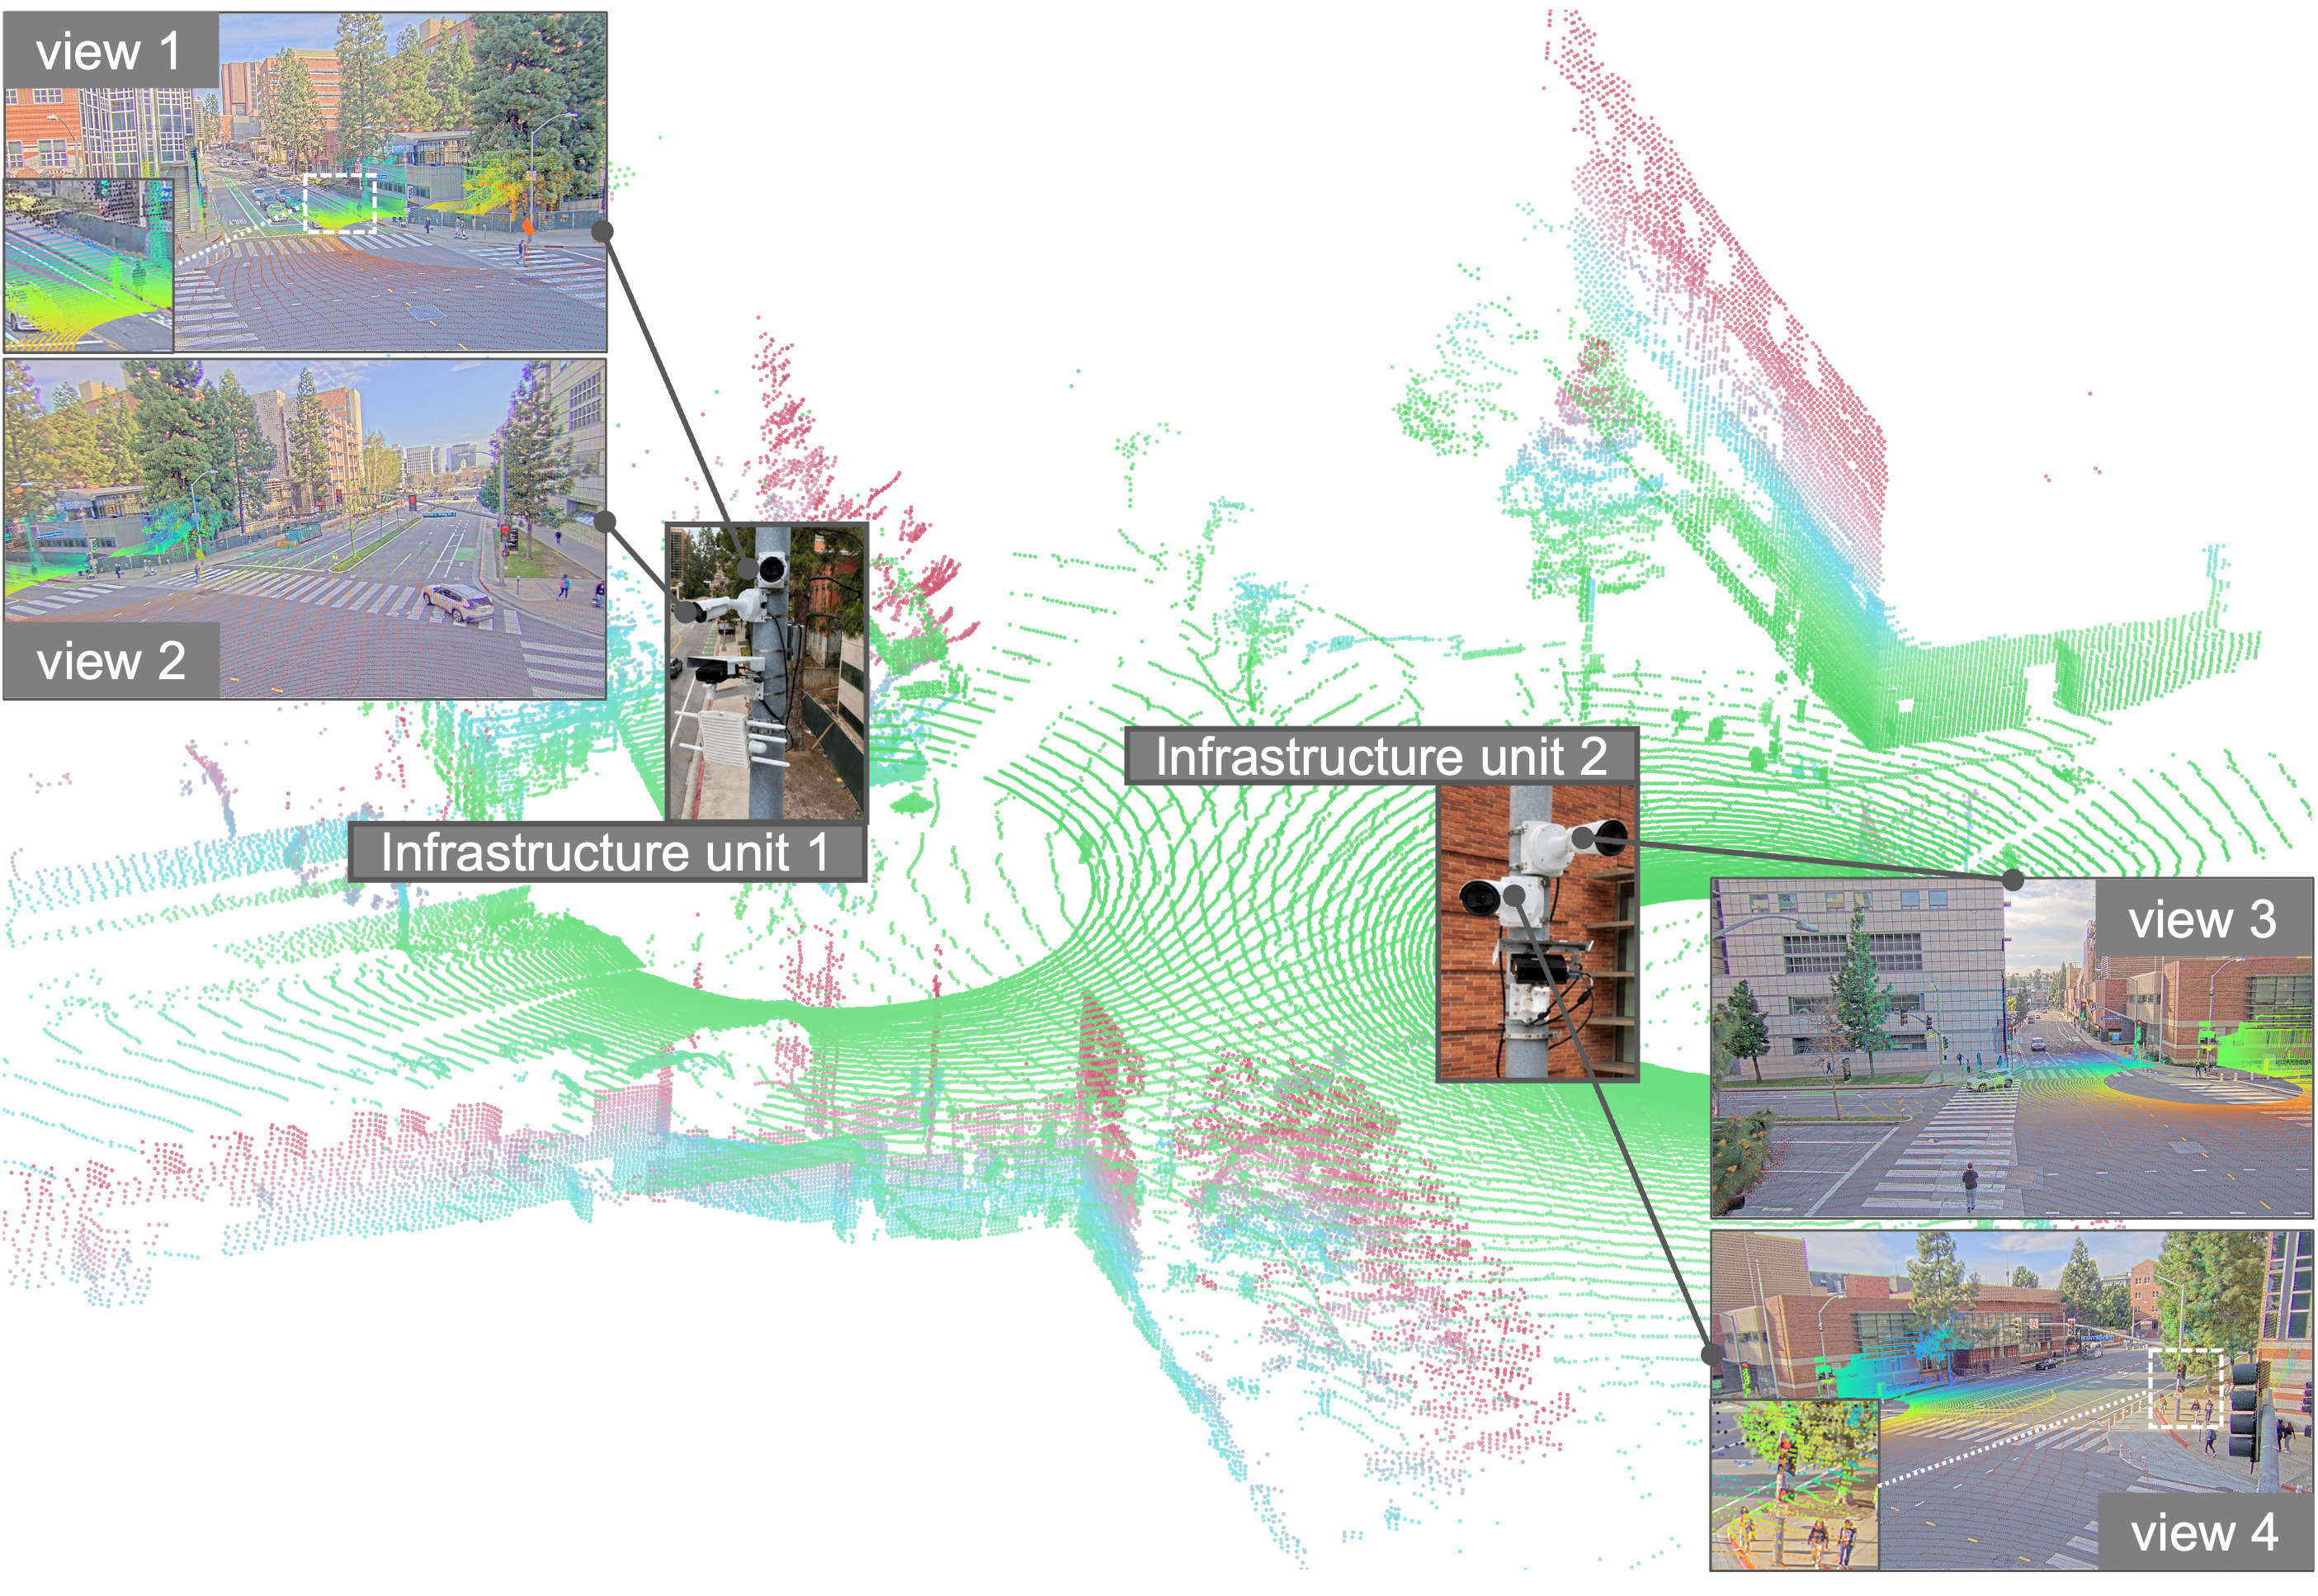
\includegraphics[width=\linewidth]{Fig1-sensor-setup.png}
  \caption{Infrastructure-side sensor configuration. Two fixed units provide
  four synchronized cameras and two LiDARs calibrated to a common roadside
  frame.}
  \vspace{-10pt}
  \label{fig:sensor_setup}
\end{wrapfigure}

InfraOcc reorganizes synchronized V2X-Real streams from object-level
cooperative perception into dense roadside occupancy supervision
\citep{InfraOcc}. Two fixed infrastructure units each carry one LiDAR and two
high-resolution cameras under GPS time synchronization. Calibration maps the
four camera streams, two point clouds, and occupancy annotations into a common
roadside coordinate system. The four cameras are the only exteroceptive model
inputs. LiDAR is used solely for benchmark construction and ground-truth
generation. Thus the reported setting remains camera-only despite the
multimodal data-collection platform.

Roadside benchmarks such as Rope3D and DAIR-V2X also study fixed or cooperative
perception \citep{Rope3D,DAIRV2X}, but primarily evaluate object-level
detection. InfraOcc instead retains a fixed coordinate system for dense
occupancy, exposing voxel-level persistence and displacement. This property is
essential for testing whether a current voxel retrieves its historical feature
from a source-consistent location.

\subsection{Benchmark Scope and Construction Contract}
\label{sec:benchmark_contract}

InfraOcc provides a real-world protocol that combines fixed roadside sensing,
temporally continuous dense semantic voxel labels, and camera-only evaluation.
Ego-centric occupancy benchmarks assume a moving sensor frame, while existing
roadside and cooperative datasets predominantly expose object-level detection
or tracking labels. We therefore use the InfraOcc protocol for primary
evaluation and complement it with matched P/T/R transfer to two temporal
occupancy backbones.

The benchmark contains 290 temporally continuous roadside sequences, with 215
used for training and 75 for evaluation. Each sequence spans approximately
10--24 seconds. Raw streams are captured at 10 Hz and dense occupancy is labeled
at 2 Hz, giving the 0.5 s interval used by RoadOcc. Each keyframe contains four
calibrated camera views and a semantic occupancy volume over
$[-64,64]\times[-64,64]\times[-4.8,1.6]$ m at 0.4 m resolution, or
$320\times320\times16$ voxels. Labels distinguish occupied, free, and
unobserved space; unobserved voxels are excluded from supervision and
evaluation.

Occupancy construction separates persistent structure from transient objects.
A semantic static scaffold is accumulated from registered vehicle-side LiDAR
after dynamic-point removal. Dynamic geometry is reconstructed from
infrastructure-side LiDAR using annotated object tracklets, box-guided alignment,
and local registration. The two sources are recomposed at each keyframe in the
fixed roadside frame and voxelized. Ray traversal labels free space before the
first observed surface, while voxels behind surfaces or outside valid rays remain
unobserved. These LiDAR sources construct supervision only; RoadOcc receives no
LiDAR feature as model input.

\begin{figure}[t]
  \centering
  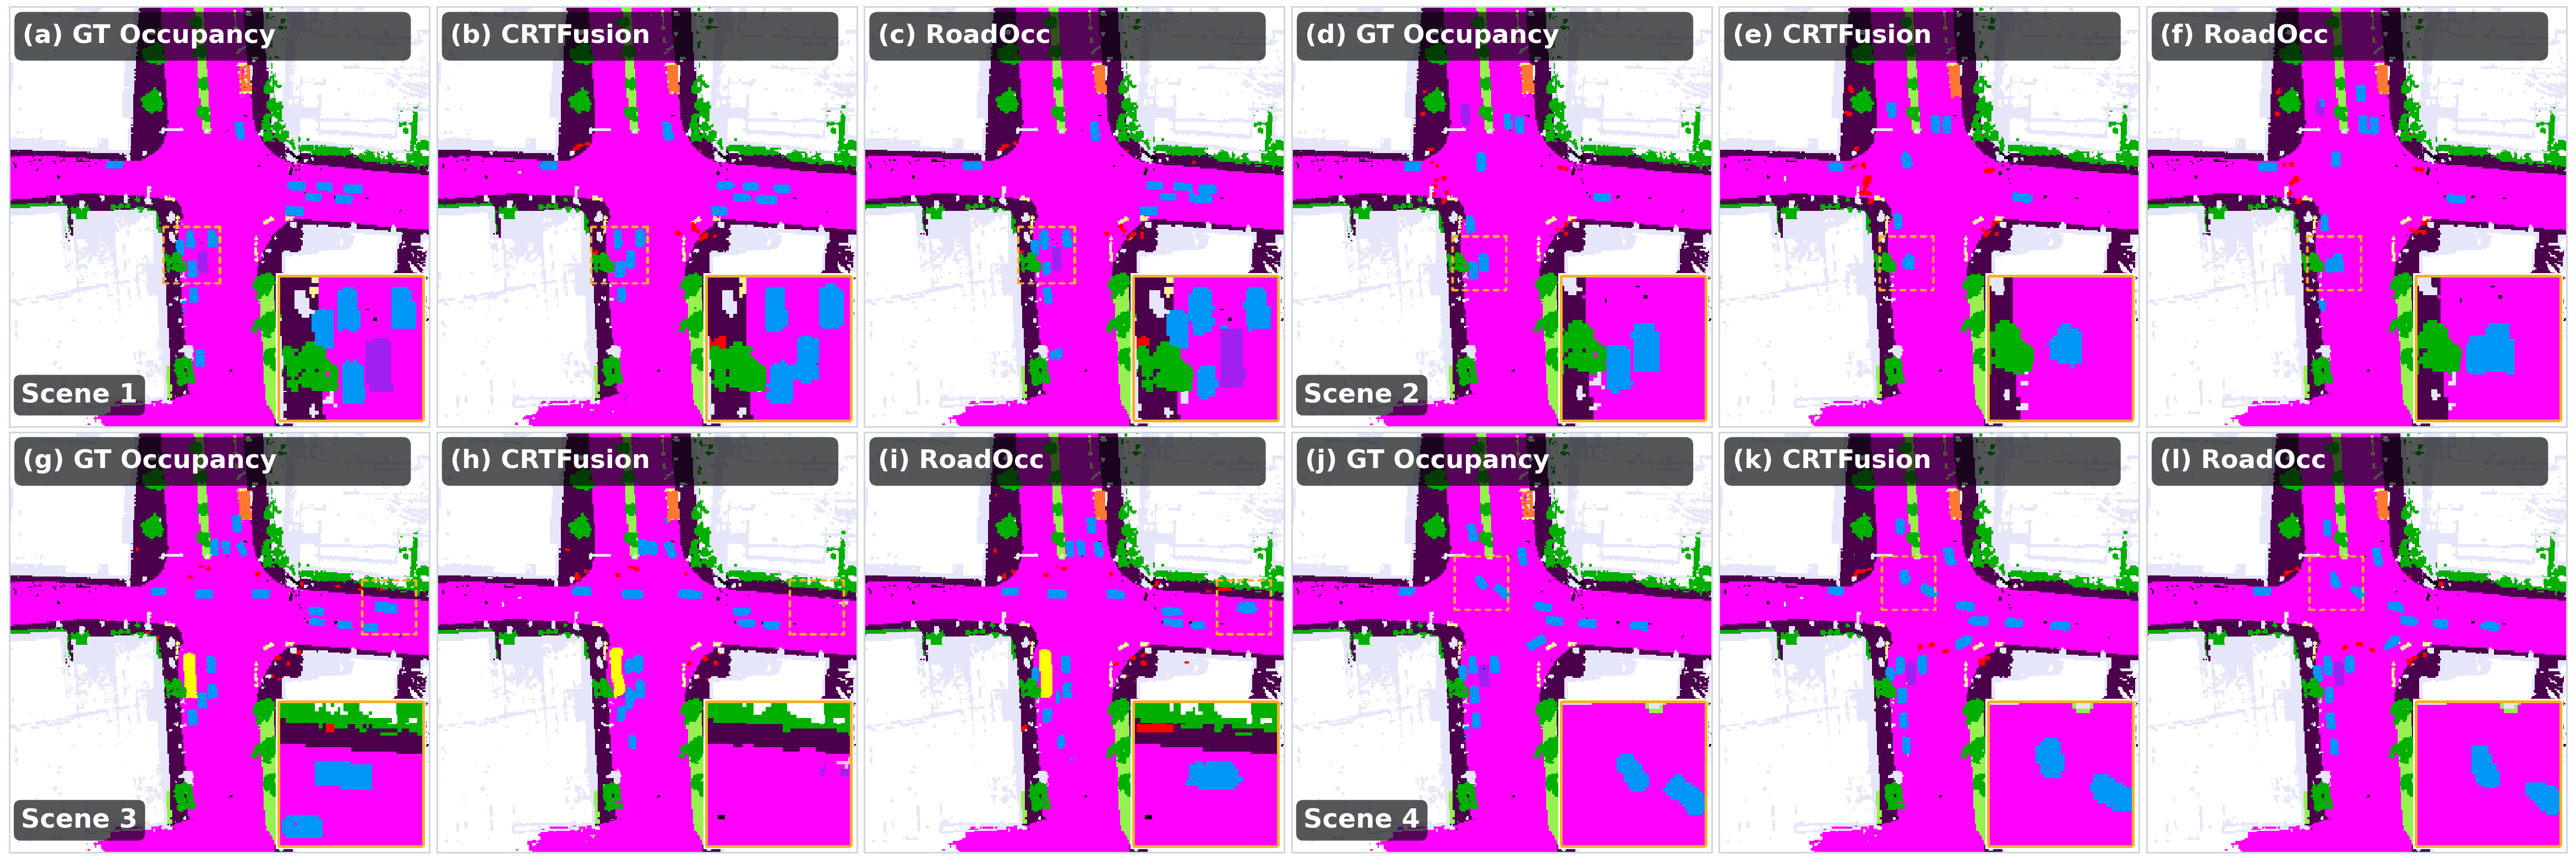
\includegraphics[width=\linewidth]{Fig2-comparison.png}
  \caption{Matched-token occupancy comparison across four scenes. Each triplet
  shows GT, CRT-Fusion, and RoadOcc in a common BEV frame and semantic palette.
  The lower-right insets enlarge a representative region that RoadOcc recovers
  but CRT-Fusion mispredicts.}
  \label{fig:supp_crtfusion}
\end{figure}

\noindent\textbf{Qualitative occupancy recovery.}
Figure~\ref{fig:supp_crtfusion} compares both methods on identical tokens and
coordinates. In the highlighted regions, CRT-Fusion either omits a participant
or assigns an incorrect footprint, whereas RoadOcc more closely follows the GT
extent and class. The surrounding road structure remains visually unchanged.
The gain is therefore concentrated on transient participants rather than
obtained by altering the dominant static background.

\subsection{Velocity-Target Construction}
\label{sec:velocity_target_contract}

InfraOcc occupancy labels do not by themselves define the transport field used
by RoadOcc. We therefore generate planar voxel-velocity targets from annotated
dynamic boxes and their temporal tracklets. Raw box velocity and adjacent-frame
tracklet displacement provide two candidates in the fixed roadside frame.

For track $j$, let $\mathbf R_{\rm rs\leftarrow raw}$ transform planar vectors
from the annotation frame into the fixed roadside frame, and let
$\mathbf c_{j,t}^{\rm rs}$ be its roadside-frame center. The two candidate
velocities are
\begin{equation}
 \widetilde{\mathbf v}_{j,t}
 =\mathbf R_{\rm rs\leftarrow raw}\mathbf v^{\rm raw}_{j,t},
 \qquad
 \mathbf d_{j,t}
 =\frac{\mathbf c_{j,t+\Delta t}^{\rm rs}-\mathbf c_{j,t}^{\rm rs}}{\Delta t},
 \qquad \Delta t=0.5\ \mathrm{s}.
 \label{eq:supp_velocity_candidates}
\end{equation}
We denote the selected candidate by $\overline{\mathbf v}_{j,t}$. A valid
tracklet displacement replaces the raw estimate when the raw estimate is
invalid, when their speeds differ by at most $10\ \mathrm{m/s}$, or when their
speed ratio is at most two.
The corrected velocity is rasterized over dynamic occupancy inside each box,
whose vertical extent is expanded by a factor of 1.5 to absorb sparse boundary
misalignment. Let $\widetilde B_{j,t}$ denote this expanded box. The native
target assigned to a dynamic voxel is
\begin{equation}
 \mathbf v_t^{\rm gt}(\mathbf x)=
 \begin{cases}
 \mathbf 0, & \|\overline{\mathbf v}_{j,t}\|_2<0.8\ \mathrm{m/s},\\
 \operatorname{clip}_{60}\!\left(\overline{\mathbf v}_{j,t}\right),
 & \mathbf x\in\widetilde B_{j,t}\cap\mathcal O_{t}^{\rm dyn},
 \end{cases}
 \label{eq:supp_velocity_rasterization}
\end{equation}
where $\operatorname{clip}_{60}$ limits the magnitude to $60\ \mathrm{m/s}$.
For candidates no faster than 2 m/s, a one-step ($0.5$ s)
future-occupancy check compares zero-motion and transported same-class support.
The check is applied only with at least eight support voxels; zero motion is
selected when its score exceeds the transported score by at least 0.05.
Finally, face-connected component repair propagates valid motion within the
corresponding raw dynamic occupancy component, and targets are generated at
native, $1/2$, $1/4$, and $1/8$ scales.

Future occupancy is used only to construct offline supervision and evaluation
targets. Neither future images nor future features are provided to RoadOcc at
training or inference time. The two velocity thresholds serve different roles.
The 0.8 m/s threshold denoises the physical target, whereas
$\epsilon=10^{-3}$ m/s is the numerical zero test used by the P/T/R rule after
target construction.

\section{Evaluation Contract}
\label{sec:metrics}

Aggregate occupancy is dominated by persistent structure and can therefore
conceal missed or stale traffic participants. Standard protocols emphasize
semantic and geometric IoU \citep{OpenOccupancy,Occ3D2023}, whereas dynamic
occupancy and flow require motion-aware diagnostics
\citep{Cam4DOcc,LetOccFlow}. Table~\ref{tab:supp_metric_contract} formalizes our
evaluation contract on InfraOcc \citep{V2XReal,InfraOcc}. Dynamic and next-frame
IoU measure semantic recovery at the current and flow-advected next-frame
locations. Direct MAVE
and DSR jointly measure motion accuracy and coverage. Static, geometric, and ray
metrics measure whether dynamic recovery preserves the fixed scene. Together,
these diagnostics distinguish improved correspondence from reduced dynamic
support or retained stale evidence.

\begin{figure*}[t]
  \centering
  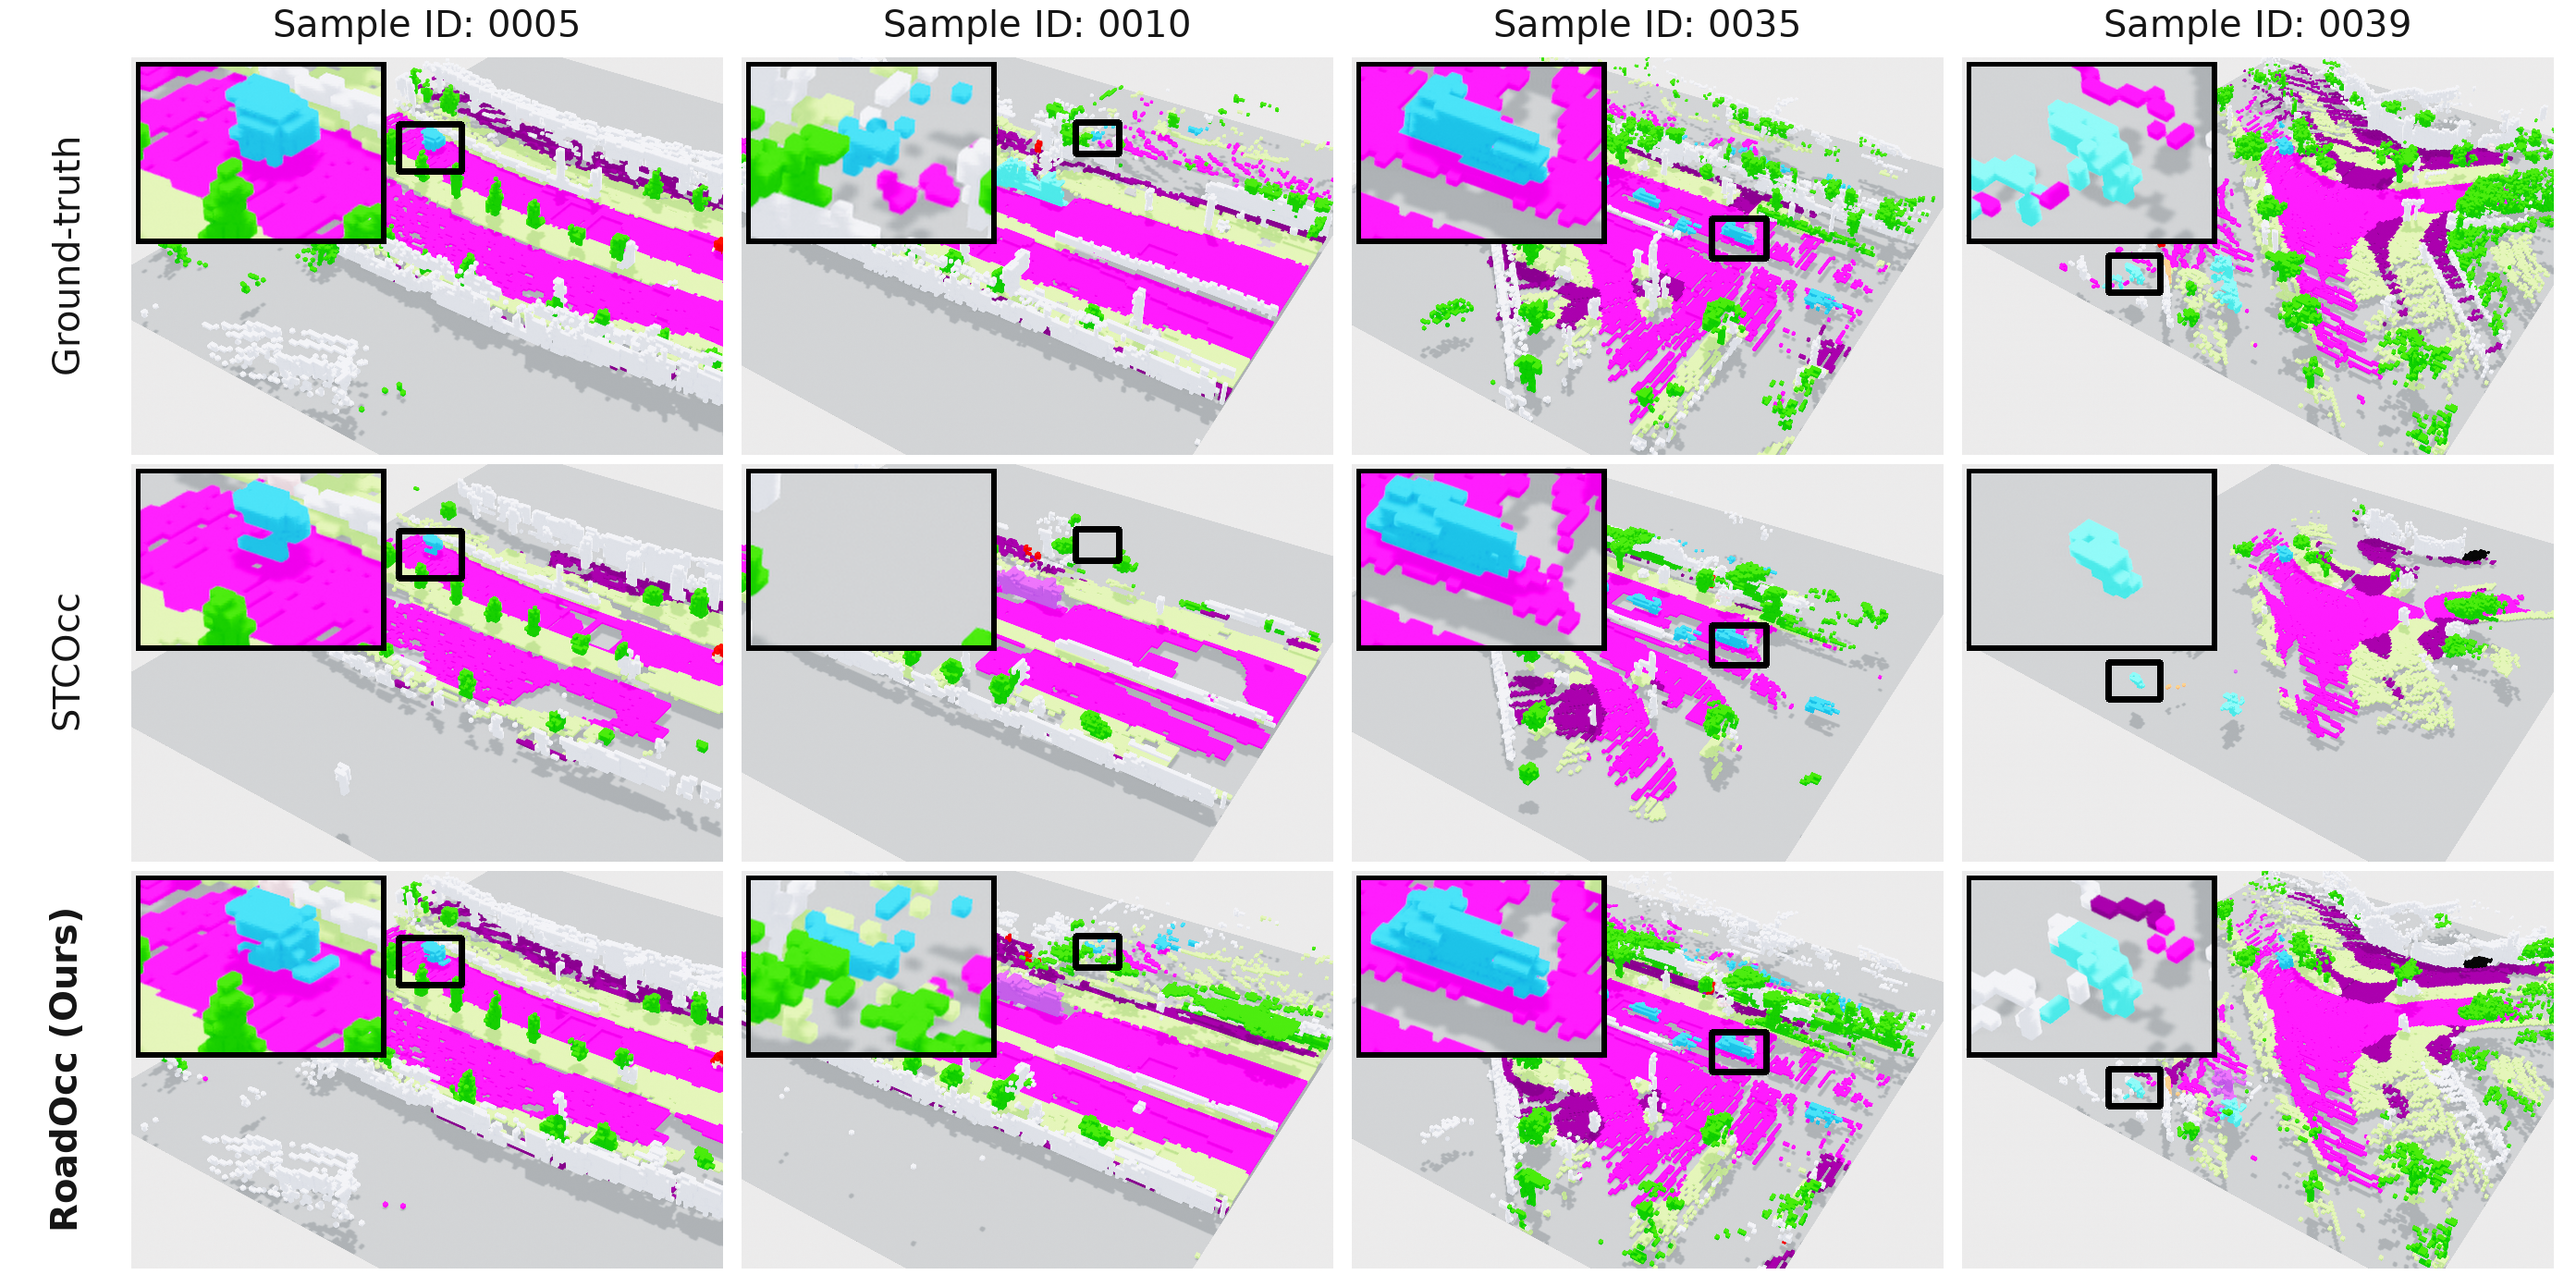
\includegraphics[width=\textwidth]{supplementary/Fig3-occ3d-comparison.png}
  \caption{\textbf{Qualitative comparison on Occ3D-nuScenes.}
  We show four validation frames under the official camera-visible mask,
  semantic palette, voxel grid, and viewing transform. Black boxes and the
  upper-left insets show the same GT dynamic component in all three rows.
  Each region is selected where RoadOcc recovers more of that component than
  the released STCOcc checkpoint.}
  \label{fig:supp_occ3d_comparison}
\end{figure*}

\noindent\textbf{Dynamic-object comparison.}
From left to right, RoadOcc raises recall within the highlighted GT component
from 58.5 to 92.5, 0.0 to 87.5, 76.4 to 92.7, and 59.0 to 90.2\%, respectively.
The insets show the corresponding recovery of missed or truncated traffic
participants.

\begin{table}[h]
  \belowrulesep=0pt
  \aboverulesep=0pt
  \centering
  \footnotesize
  \caption{Metric and diagnostic scope.}
  \label{tab:supp_metric_contract}
  \renewcommand{\arraystretch}{1.05}
  \setlength{\tabcolsep}{0pt}
  \begin{tabular*}{\textwidth}{@{\extracolsep{\fill}}llll@{}}
    \toprule[1.0pt]
    \multicolumn{1}{c}{Metric} & \multicolumn{1}{c}{Support} &
    \multicolumn{1}{c}{Failure} & \multicolumn{1}{c}{Role} \\
    \midrule
    Dyn. mIoU $\metricup$ & Dynamic GT voxels & Omission / class error & Dynamic semantic recovery \\
    Static / gIoU $\metricup$ & Static / occupied support & Static-structure damage & Static-scene guardrail \\
    Next Dyn. $\metricup$ & Advected dynamic GT & Displacement error & Next-frame consistency \\
    Direct MAVE $\metricdown$ & All dynamic GT voxels & Miss-induced motion bias & Unconditional flow error \\
    TP-MAVE $\metricdown$ / DSR $\metricup$ & Matched semantics / dynamic GT & Conditional-match bias & Matched accuracy / coverage \\
    RayIoU $\metricup$ & Visible evaluation rays & Surface-depth mismatch & Geometric fidelity \\
    \bottomrule
  \end{tabular*}
\end{table}



Direct MAVE evaluates every valid GT dynamic voxel, whereas TP-MAVE is
conditional on a correct semantic match and must therefore be interpreted with
DSR. A valid routing improvement should increase dynamic IoU and DSR, decrease
Direct MAVE, and preserve the static and geometric guardrails. Reporting these
quantities together distinguishes improved semantic correspondence from a lower
conditional error caused by reduced semantic support.
For completeness, let $\mathcal D$ be the set of evaluated dynamic classes,
$V_c=\{i:y_i=c\}$ the valid GT voxels of class $c$, and
$V_c^{\rm TP}=\{i\in V_c:\widehat y_i=c\}$. Classes without valid support are
omitted from the corresponding class macro-average; $\mathcal D'$ and
$\mathcal D''$ denote the supported classes for Direct and TP-MAVE,
respectively. The two velocity metrics and semantic recall are
\begin{align}
 \mathrm{Direct\ MAVE}
 &=\frac{1}{|\mathcal D'|}\sum_{c\in\mathcal D'}
   \frac{1}{|V_c|}\sum_{i\in V_c}
   \|\widehat{\mathbf v}_i-\mathbf v_i\|_2,\\
 \mathrm{TP\mbox{-}MAVE}
 &=\frac{1}{|\mathcal D''|}\sum_{c\in\mathcal D''}
   \frac{1}{|V_c^{\rm TP}|}\sum_{i\in V_c^{\rm TP}}
   \|\widehat{\mathbf v}_i-\mathbf v_i\|_2.
\end{align}
Thus MAVE is class-macro while DSR is a micro recall over GT dynamic voxels.
For next-frame dynamic IoU, centers of predicted current dynamic voxels are
advanced by the predicted planar velocity for $0.5$ s, transformed to the next
roadside frame, and voxelized. Collisions use deterministic per-class majority
assignment before class-macro IoU is computed against next-frame GT. This
flow-advected diagnostic is distinct from the same-class radius-one hit score
used only in the backwarp visualization.
\begin{align}
\mathrm{DSR}
&=\frac{\sum_{c\in\mathcal D}|V_c^{\rm TP}|}
        {\sum_{c\in\mathcal D}|V_c|}.
\end{align}



\section{Occ3D-nuScenes Transfer}
\label{sec:occ3d_nuscenes}

\begin{wraptable}[11]{r}{0.62\columnwidth}
  \vspace{-5pt}
  \belowrulesep=0pt
  \aboverulesep=0pt
  \centering
  \footnotesize
  \caption{Mask-trained comparison on Occ3D-nuScenes. All metrics are percentages.}
  \label{tab:occ3d_nuscenes}
  \setlength{\tabcolsep}{0pt}
  \renewcommand{\arraystretch}{1.05}
  \begin{tabular}{@{}C{2.40cm}C{1.10cm}C{1.35cm}C{0.80cm}C{1.55cm}C{1.45cm}@{}}
    \toprule
    Method & BB & Res. & mIoU & Dynamic mIoU & Static mIoU \\
    \midrule
    FB-Occ & R50 & 256$\!\times\!$704 & 39.10 & 33.75 & 43.89 \\
    ViewFormer & R50 & 256$\!\times\!$704 & 41.90 & 35.00 & 47.93 \\
    COTR & R50 & 256$\!\times\!$704 & 44.50 & 38.60 & 49.63 \\
    ALOcc & R50 & 256$\!\times\!$704 & 41.40 & 35.40 & 46.73 \\
    STCOcc & R50 & 256$\!\times\!$704 & 44.60 & 39.01 & 49.58 \\
    \method{} & R50 & 256$\!\times\!$704 & \textbf{45.01} & \textbf{39.80} & \textbf{49.64} \\
    \bottomrule
  \end{tabular}
\end{wraptable}

Table~\ref{tab:occ3d_nuscenes} compares representative camera-only temporal
methods under the mask-trained Occ3D-nuScenes protocol~\citep{Occ3D2023,FBOCC,ALOcc,ViewFormer,COTR,STCOcc}.
Dynamic mIoU averages the eight traffic-participant classes, while static mIoU
averages the remaining nine occupied classes. We compute both group metrics
from published per-class IoUs when available. ALOcc directly reports dynamic
mIoU; its static mIoU follows from its reported dynamic and overall mIoUs.
Before rounding, the three aggregates satisfy
$\mathrm{mIoU}=(8\,\mathrm{Dyn.}+9\,\mathrm{Sta.})/17$.
RoadOcc leads all three aggregates, improving STCOcc by 0.41 overall, 0.79
dynamic, and 0.06 static mIoU points. The larger dynamic gain shows that
motion-aware routing transfers without sacrificing static-scene accuracy.


\section{Training Objectives}
\label{sec:training_objectives}
\begin{figure}[t]
  \centering
  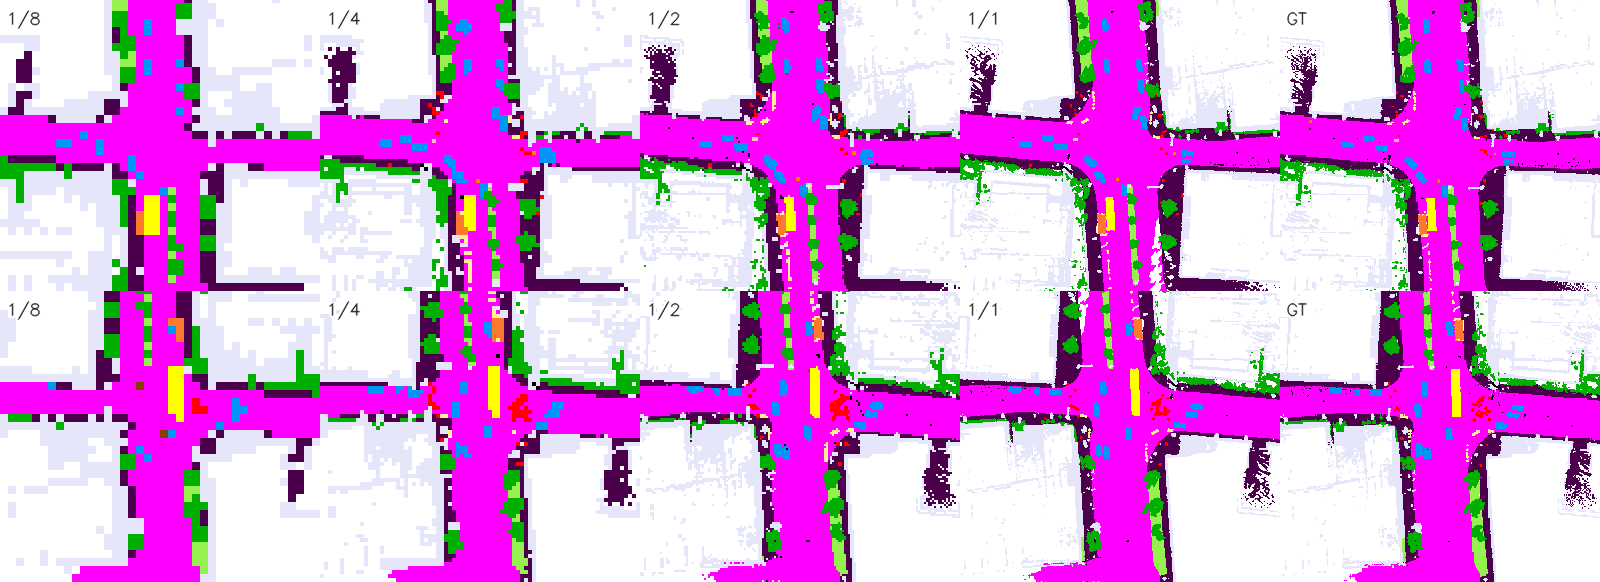
\includegraphics[width=\textwidth]{Fig4-recursive.png}
  \caption{Coarse-to-fine occupancy decoding for two representative samples.
  Columns show predictions from $1/8$ scale through full resolution and the
  corresponding GT. Successive stages sharpen road boundaries and recover
  traffic participants that remain unresolved at coarse resolution.}
  \label{fig:supp_recursive_decoding}
\end{figure}
RoadOcc assigns each loss to one decision in the DCA--VVE--VDSF chain.
Camera-depth supervision uses weight $0.5$. Semantic occupancy is supervised
from full resolution to $1/8$ scale with weights $[1.0,0.5,0.25,0.125]$, while
the static, dynamic, and DCA-candidate auxiliaries each use $0.5$. VVE receives
class- and speed-balanced robust flow supervision at all four scales with weight
$0.1$. Its local-connectivity term also uses $0.1$ and starts after epoch 3 to
limit noisy early correspondences.
The P/T/R route loss spans the native, $1/2$, $1/4$, and $1/8$ scales with
relative weights $[1,0.5,0.25,0.125]$, normalized under
$\lambda_{\rm route}=0.5$. Each scale constructs the semantic-support target
using its physical cell size. Equal-class-weight cross-entropy is augmented from
epoch 2 by a soft-overlap term of weight $0.5$ with state weights
$[1,1,0.25]$. Each executed routing field therefore receives
resolution-matched supervision.


\subsection{Candidate, Motion, and Routing Contract}
\label{sec:exact_contract}

\noindent\textbf{DCA score.}
Let $\boldsymbol\pi_{\rm cur}$ and $\boldsymbol\pi_{\rm sta}$ denote current
and static-reference class probabilities, and let
$\mathcal C_{\rm sta}^{+}$ contain the static classes together with empty
class. The executed
change and dynamic scores are
\begin{align}
 \delta(\mathbf x)&=\frac{1}{|\mathcal C_{\rm sta}^{+}|}
 \sum_{c\in\mathcal C_{\rm sta}^{+}}
 |\pi_{{\rm cur},c}(\mathbf x)-\pi_{{\rm sta},c}(\mathbf x)|,\\
 p_{\rm dyn}(\mathbf x)&=\sum_{c\in\mathcal C_{\rm dyn}}
 \pi_{{\rm cur},c}(\mathbf x),\\
 c(\mathbf x)&=\frac{\max\{\delta(\mathbf x),p_{\rm dyn}(\mathbf x)\}}
 {\max_{\mathbf y}\max\{\delta(\mathbf y),p_{\rm dyn}(\mathbf y)\}+10^{-6}}.
\end{align}
DCA ranks this normalized score. Before fixed top-$K$ selection, VDSF uses
$\operatorname{clip}(c+0.5e,0,1)$, where $e$ is nonempty support and hence
$\eta=0.5$ in Eq.~\ref{eq:vdsf_selection}. For an anchor
$\mathbf r=(\mathbf x,z_{\mathbf r})$, $c(\mathbf r)$ is the score of the
corresponding voxel-height bin and is shared across cameras before visibility
masking. Let $d_{n,\mathbf r}$ be its projected depth, $\widehat d_n$ the
winning predicted depth bin, and $\Delta_d=1$ m the bin width. The executed
depth-consistency factor is
\begin{equation}
 \beta_{n,\mathbf r}=\exp\!\left[-\frac{\sigma^2}{2}
 \min_{\xi\in\{-\Delta_d,+\Delta_d\}}
 \left|d_{n,\mathbf r}-(\widehat d_n+\xi)\right|^2\right],
 \qquad \sigma=2.
\end{equation}
Deformable-attention weights are first softmax-normalized over sampled points,
then multiplied by $\beta$. They are not renormalized afterward; camera
outputs are averaged over cameras retaining at least one visible anchor.




\begin{figure}[t]
  \centering
  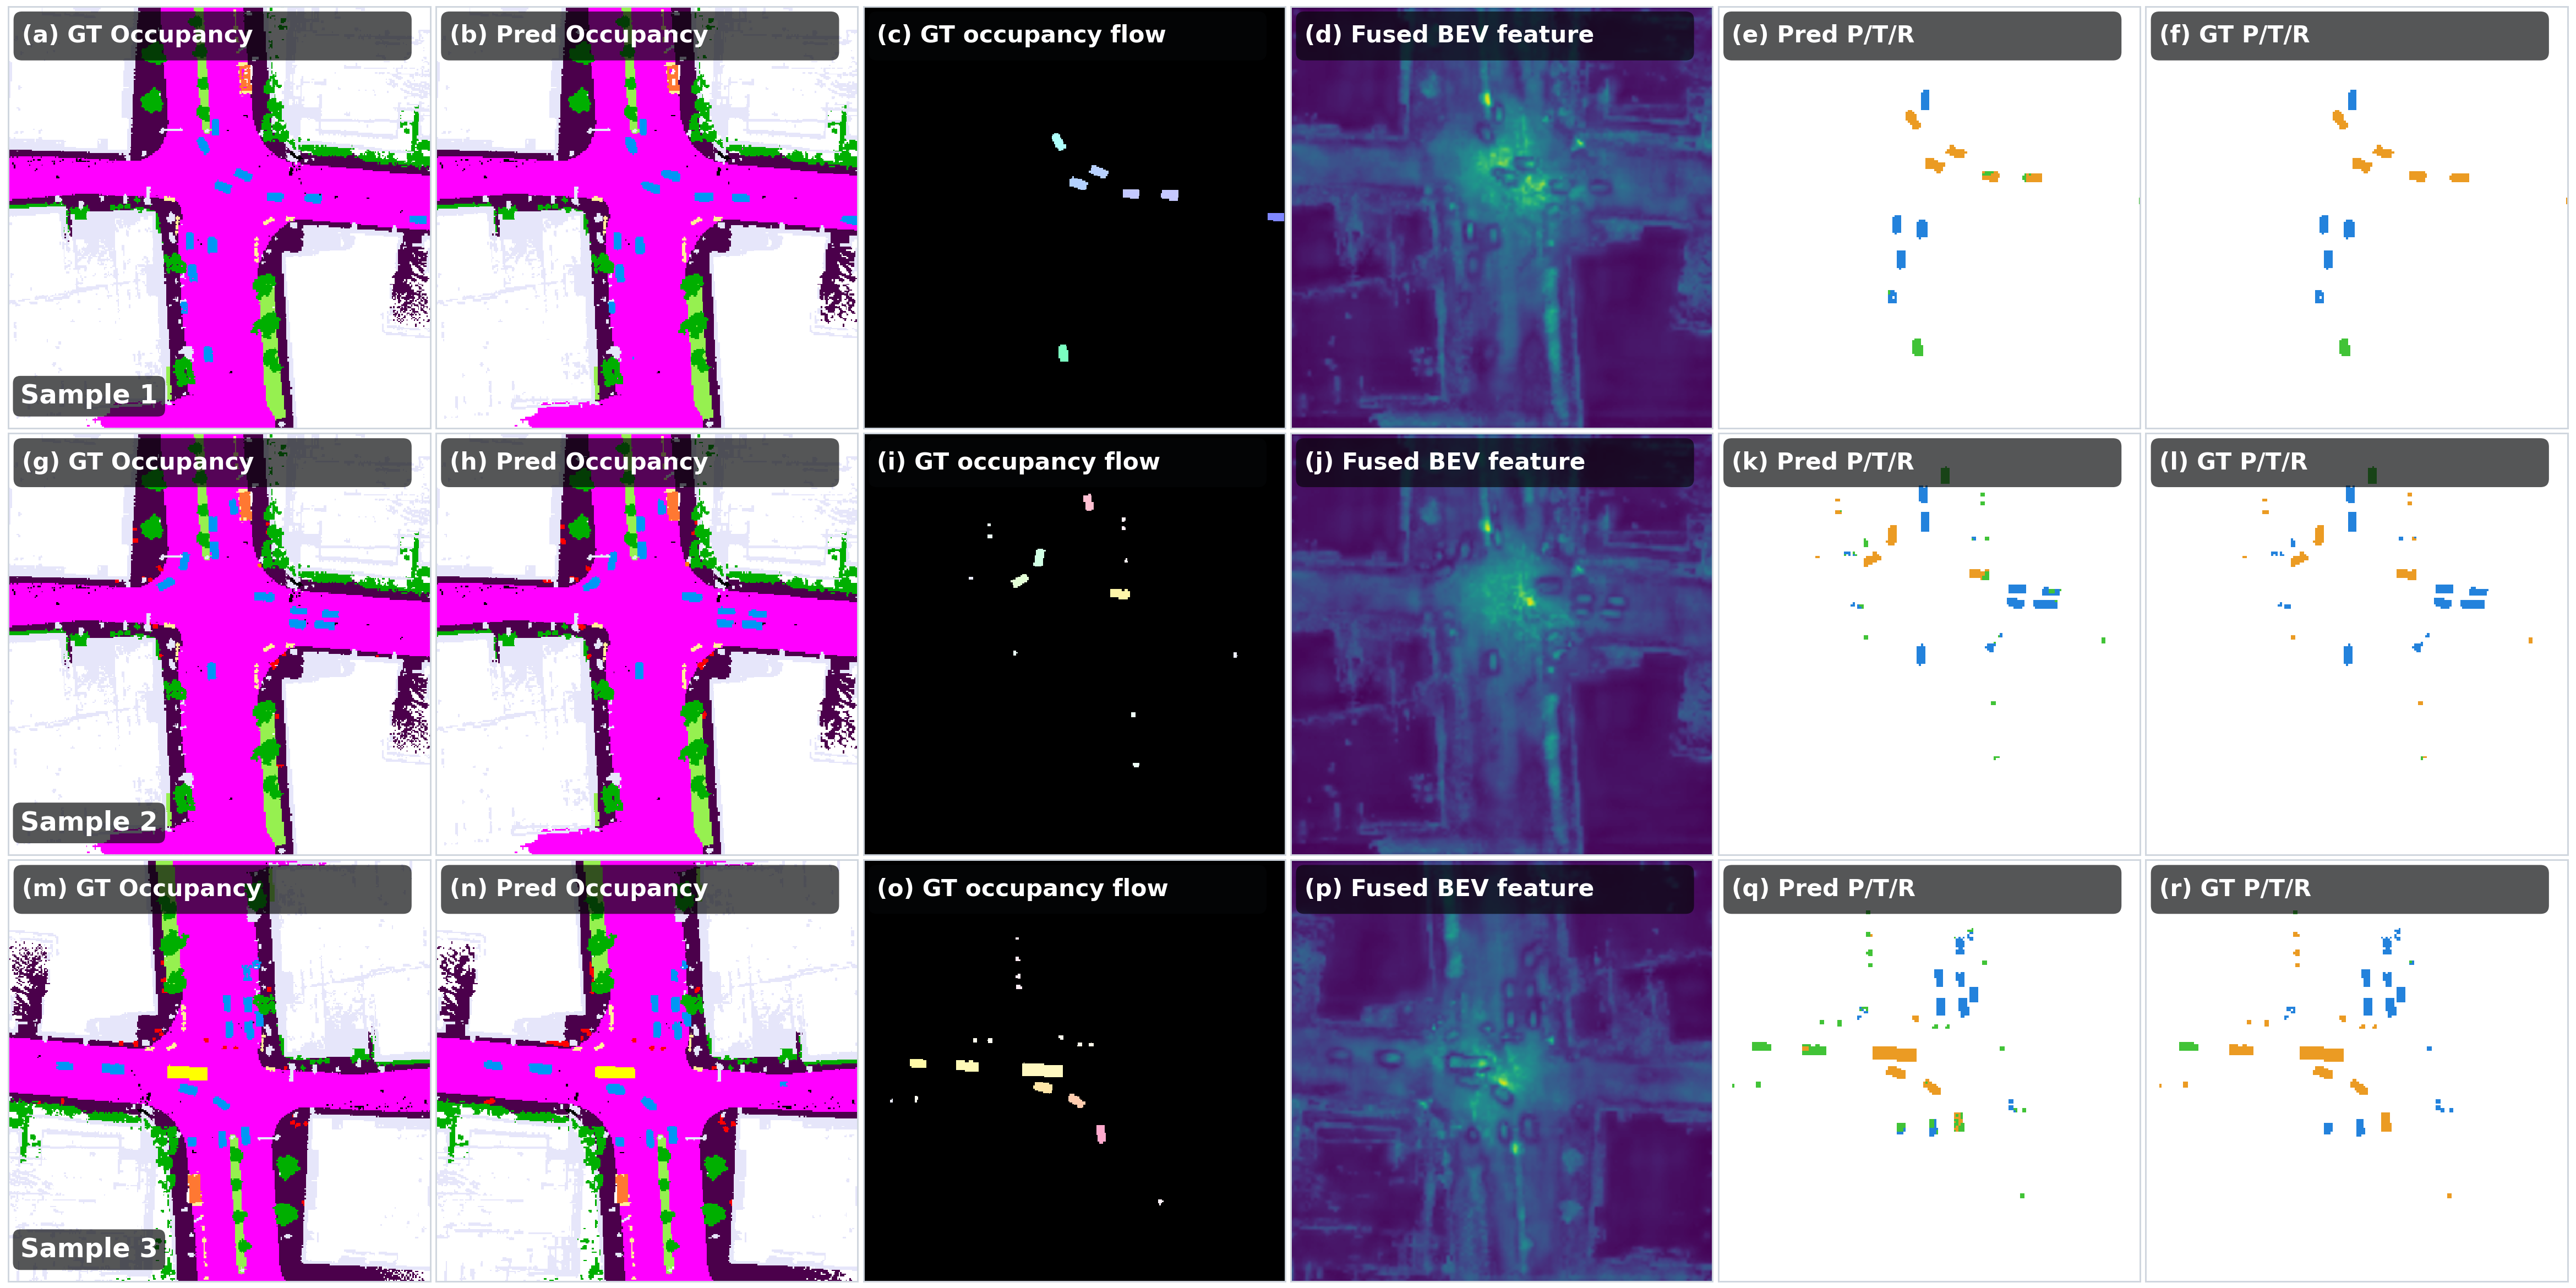
\includegraphics[width=\linewidth]{Fig5-ptrnative.png}
  \caption{Native-scale P/T/R routing across three samples. Predicted and GT
  routes share GT dynamic support. Blue, orange, and green denote Persist,
  Transport, and Refresh, respectively.}
  \label{fig:supp_ptr_prediction}
\end{figure}



\noindent\textbf{Recursive occupancy decoding.}
Figure~\ref{fig:supp_recursive_decoding} shows the progressive output of the
multi-scale decoder. Coarse predictions establish scene layout, while finer
stages restore object boundaries and sparse traffic participants before the
full-resolution output.

\noindent\textbf{VVE correspondence range.}
At scales $1/8$, $1/4$, and $1/2$, the $5\times5$ correlation volume
($r=2$) spans $\pm6.4$, $\pm3.2$, and $\pm1.6$ m on the native $0.4$ m grid.
Over the $0.5$ s interval, the equivalent speed ranges are twice these values.

Each correlation operand is normalized to unit $\ell_2$ norm with
$\epsilon=10^{-6}$. The resulting volume has 25 channels and is concatenated
with current and historical BEV embeddings, processed by two $3\times3$
convolution blocks, and decoded as a two-dimensional velocity residual in m/s.
The window bounds only the
explicit matching evidence. The coarse velocity is
added to each finer prediction and the final continuous residual is not clipped,
so it does not impose a hard bound on predicted speed. The GT-flow study in the
main paper isolates the value of transport addresses across speed ranges. In
the temporal blend, the history branch receives weight
$0.5\,\mathbf 1_{\rm hist}\max_z p_{\rm dyn}(\mathbf x,z)$; this is current
dynamic support gated by history validity, rather than a calibrated measure of
historical correspondence.

\noindent\textbf{Native P/T/R target.}
For a current dynamic voxel, the Transport source is
\begin{equation}
 \mathbf x_{\rm src}=\operatorname{round}\!\left(
 \mathbf x-\frac{\Delta t\,\mathbf v_t(\mathbf x)}{0.4\ \mathrm m}\right),
 \qquad \Delta t=0.5\ \mathrm s.
\end{equation}
Persist tests the fixed-coordinate address and Transport tests $\mathbf x_{\rm src}$.
Support means that the nearest previous GT contains the same semantic class at
the same height within a $3\times3$ XY neighborhood ($L_\infty$ radius one).
Support is Boolean. One or more matching voxels suffice, with no instance-level
tie-breaking.
Out-of-grid or unsupported candidates are assigned Refresh rather than removed.
The target follows InfraOcc's voxel-level semantic supervision and therefore
tests class-consistent support without requiring instance identities.

\noindent\textbf{Coarse-to-fine FIFO routing.}
At each decoder scale, a shared controller projects current features and the
nearest fixed-coordinate history to eight channels, adds embeddings of detached VVE flow
(normalized by 10 m/s) and detached upsampled coarse P/T/R, and predicts three
route logits after a $3\times3\times3$ refinement. A lightweight native head
combines upsampled $1/2$ context, native flow, and the finest P/T/R distribution
for full-resolution routing. Each scale shares its route distribution across
valid FIFO slots, whose ages and cached VVE fields determine source-consistent
inverse-trajectory Transport addresses. Routed slots are concatenated before
fusion. Invalid slots are masked and queues reset at scene boundaries. Fusion
uses soft routes, with argmax only for diagnostics.


\section{Capacity and Efficiency Context}
\label{sec:model_size}

\begin{wraptable}[5]{r}{0.50\columnwidth}
  \vspace{-5pt}
  \belowrulesep=0pt
  \aboverulesep=0pt
  \centering
  \footnotesize
  \caption{Accuracy--efficiency comparison.}
  \label{tab:capacity_efficiency}
  \setlength{\tabcolsep}{2.0pt}
  \renewcommand{\arraystretch}{1.05}
  \begin{tabular}{@{}L{2.20cm}|C{1.00cm}C{1.00cm}|C{1.00cm}C{1.00cm}@{}}
    \toprule[1.0pt]
    Setting & Params.$\downarrow$ & Lat.$\downarrow$ & All$\uparrow$ & Dyn.$\uparrow$ \\
    \midrule
    % BEVDet~'21 & 100.66 & 41.92 & 45.14 & 21.19 \\
    % BEVFormer~'22 & 69.21 & 180.59 & 47.76 & 10.73 \\
    % BEVDepth~'23 & 100.66 & 57.43 & 46.81 & 19.64 \\
    % TPVFormer~'23 & 80.76 & 134.63 & 43.09 & 4.36 \\
    % SurroundOcc~'23 & 80.04 & 44.40 & 50.77 & 11.37 \\
    % CONet~'23 & 100.74 & 53.23 & 49.25 & 18.93 \\
    % SparseOcc~'24 & 105.08 & 64.30 & 45.42 & 9.41 \\
    % GaussianFormer~'24 & 36.32 & 65.50 & 43.63 & 10.45 \\
    % CRT-Fusion~'24 & 56.82 & 106.22 & 53.83 & 27.02 \\
    STCOcc~'25 & 60.47 & 333.44 & 60.85 & 27.66 \\
    RoadOcc (\textbf{ours}) & 78.69 & 253.25 & 65.29 & 32.37 \\
    \bottomrule
  \end{tabular}
  \vspace{-5pt}
\end{wraptable}
Table~\ref{tab:capacity_efficiency} reports parameters, synchronized model
latency measured on a single NVIDIA RTX A6000 with batch size 1, and occupancy
accuracy for the reproduced temporal configurations.
Although RoadOcc contains more parameters than STCOcc, it reduces latency from
333.44 to 253.25 ms because DCA, VVE, and P/T/R operate on sparse or
low-resolution features, while the main temporal path uses shorter histories
and smaller token budgets. This efficient routing also improves all-class and
dynamic mIoU by $+$4.44 and $+$4.71 points, respectively.

\begin{wrapfigure}[17]{r}{0.50\columnwidth}
  \vspace{-15pt}
  \centering
  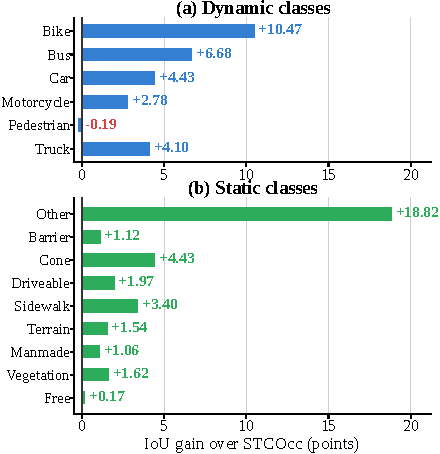
\includegraphics[width=\linewidth]{Fig6-classwise-gains.pdf}
  \caption{Class-wise IoU gains over STCOcc.}
  \label{fig:supp_classwise_gains}
  \vspace{-20pt}
\end{wrapfigure}
\noindent\textbf{Class-wise improvement.}
Figure~\ref{fig:supp_classwise_gains} resolves the official result in
Table~\ref{tab:infraocc_main_results} into dynamic and static classes. Relative
to STCOcc, RoadOcc improves five of the six dynamic classes, led by Bike at
$+$10.47 and Bus at $+$6.68, while Pedestrian changes by $-$0.19. Every static
class also improves. The category pattern therefore connects the aggregate gain
to both parts of the routing objective. Corrected addresses recover transient
participants, while source selection preserves the persistent roadside scene.


\section{Controlled Design Studies}
\label{sec:controlled}


All studies hold the backbone, data protocol, optimizer, training schedule,
scene-boundary queue reset, and VDSF configuration fixed. Unless varied explicitly,
the decoder stages use $K=[2000,512,128]$ sparse tokens and retain
$[8,4,2]$ history samples, respectively. The main paper reports the matched
address and P/T/R controls. The supplementary studies below provide
non-overlapping evidence on VVE training, route prediction, sparse allocation,
and address construction.

\noindent\textbf{Temporal-gap zero-shot generalization.}
Table~\ref{tab:supp_temporal_gap} evaluates checkpoints trained only at the
$0.5$ s cadence without fine-tuning. Phase-offset streams retain all 1,970
validation inputs, while the same 1,520 anchors with valid past and future
$1.5$ s context are scored at every gap. The elapsed time is recovered from
timestamps and used by temporal transport.

\begin{table}[H]
  \belowrulesep=0pt
  \aboverulesep=0pt
  \centering
  \footnotesize
  \caption{Temporal-gap zero-shot evaluation on matched anchors. Both
  checkpoints are trained only at a $0.5$ s interval.}
  \label{tab:supp_temporal_gap}
  \renewcommand{\arraystretch}{1.05}
  \setlength{\tabcolsep}{5.5pt}
  \begin{tabular}{@{}lccc|ccc@{}}
    \toprule[1.0pt]
    & \multicolumn{3}{c|}{Dyn. $\metricup$} &
      \multicolumn{3}{c}{Nxt. $\metricup$} \\
    \cmidrule(lr){2-4}\cmidrule(l){5-7}
    Method & $0.5$ s & $1.0$ s & $1.5$ s & $0.5$ s & $1.0$ s & $1.5$ s \\
    \midrule
    STCOcc~\citep{STCOcc} & 28.04 & 28.26 & 28.58 & 25.21 & 20.90 & 19.12 \\
    RoadOcc (\textbf{ours}) & \textbf{33.71} & \textbf{33.57} & \textbf{33.49} &
      \textbf{30.23} & \textbf{25.18} & \textbf{22.78} \\
    \bottomrule
  \end{tabular}
\end{table}

RoadOcc preserves a 4.91-point Dyn. advantage and a 3.65-point Nxt. advantage
even when the test gap triples. VVE represents displacement through a physical
velocity field, while P/T/R selects fixed-coordinate, transported, or current
evidence. Their combination therefore remains effective when elapsed time
changes rather than depending only on the observed $0.5$ s transition pattern.


\begin{wrapfigure}{r}{0.50\columnwidth}
  \centering
  \vspace{-10pt}
  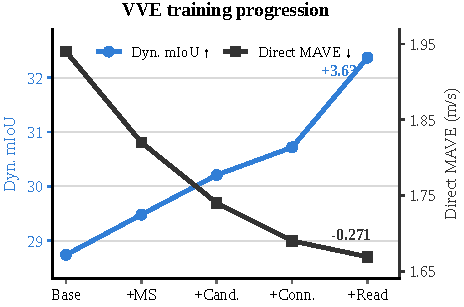
\includegraphics[width=\linewidth]{Fig7-vve-progression.pdf}
  \caption{Dynamic occupancy and motion-error progression under the VVE
  training signals.}
  \label{fig:supp_vve_progression}
  \vspace{-15pt}
\end{wrapfigure}
\noindent\textbf{VVE training design.}
The main-paper control establishes the value of reading from a corrected
address. Figure~\ref{fig:supp_vve_progression} follows a progressive sequence
that introduces multi-scale flow, candidate-map guidance, connectivity
regularization, and flow-addressed history retrieval. Dyn. improves monotonically
while Direct MAVE decreases across this progression. Overall, Dyn. rises by
$+$3.63 and Direct MAVE falls by 0.271. The final flow-addressed read contributes
another $+$1.65 Dyn. while Direct MAVE decreases by only 0.021, indicating that
its main benefit comes from retrieving useful history.

\noindent\textbf{Supported-route analysis.}
Table~\ref{tab:supp_ptr_fidelity} audits the two historical routes on valid GT
dynamic voxels. Persist emphasizes precise reuse of fixed-coordinate evidence,
while Transport provides broader coverage after displacement. Since VDSF fuses
soft probabilities over all source alternatives, these argmax statistics
characterize history reuse rather than the complete fused output. The end-to-end
effect of routing is evaluated separately through Dyn., Nxt., Direct MAVE, and
DSR.

\begin{wraptable}{r}{0.50\columnwidth}
  \belowrulesep=0pt
  \aboverulesep=0pt
  \centering
  \footnotesize
  \caption{Supported historical-route statistics on valid GT dynamic voxels.
  Percentages are computed against the full routing population.}
  \label{tab:supp_ptr_fidelity}
  \renewcommand{\arraystretch}{1.05}
  \setlength{\tabcolsep}{2.2pt}
  \begin{tabular}{@{}L{1.30cm}|C{1.25cm}C{1.25cm}|C{1.25cm}C{1.25cm}@{}}
    \toprule[1.0pt]
    State & Target & Pred. & Precision & Recall \\
    \midrule
    Persist   & 52.34 & 38.84 & 95.50 & 70.87 \\
    Transport & 44.30 & 50.40 & 72.98 & 83.03 \\
    % Refresh   &  3.36 & 10.76 & 16.87 & 54.00 \\
    \bottomrule
  \end{tabular}
  \belowrulesep=0pt
  \aboverulesep=0pt
  \centering
  \footnotesize
  \caption{Sensitivity to sparse-token allocation.}
  \label{tab:supp_token_budget}
  \renewcommand{\arraystretch}{1.05}
  \setlength{\tabcolsep}{0pt}
  \begin{tabular}{@{}C{2.50cm}|C{1.05cm}C{1.05cm}C{1.25cm}C{1.05cm}@{}}
    \toprule[1.0pt]
    Budget $K$ & Dyn. $\metricup$ & Nxt. $\metricup$ & dM $\metricdown$ & DSR $\metricup$ \\
    \midrule
    $[1000,256,64]$ & 31.74 & 30.96 & 1.716 & 60.28 \\
    $[2000,512,128]$ & 32.37 & 31.72 & 1.669 & 61.11 \\
    $[4000,1024,256]$ & 32.39 & 31.69 & 1.665 & 61.18 \\
    \bottomrule
  \end{tabular}
  \vspace{-5pt}
\end{wraptable}
\noindent\textbf{Qualitative routing behavior.}
Figure~\ref{fig:supp_ptr_prediction} relates each route to observable scene
evidence. Persist coincides with aligned objects, Transport follows nonzero
displacement, and current evidence is selected when neither historical source
is supported. Because predicted and GT routes are rendered on identical dynamic
support, their differences directly reflect source choices. The visualization
therefore audits semantic source routing independently of occupancy detection.



\noindent\textbf{Sparse-token budget.}
VDSF processes only the top-$K$ selected voxels. The token study tests whether
the reported behavior depends on a larger compute budget or on identifying the
right locations. All other model and routing settings remain fixed while $K$ is
scaled at every decoder stage.
Increasing the small allocation to the default improves Dyn. by 0.63 and DSR by
0.83. Doubling the default allocation changes Dyn. by only 0.02, dMAVE by 0.004,
and DSR by 0.07, while next-frame IoU fluctuates by $-$0.03. This saturation
shows that the reported result does not rely on continually expanding the
sparse-token budget.



\noindent\textbf{Velocity-address construction.}
Velocity is useful for fusion only when it points to evidence that explains the
current target. Table~\ref{tab:supp_address_rule} therefore compares a
fixed-coordinate read, a target-vector backtrace, and the complete source-consistent
rule under an otherwise fixed P/T/R router. This isolates address construction
from subsequent source acceptance and complements flow-based warping in prior
occupancy models \citep{LetOccFlow,STCOcc}.

\begin{wraptable}{r}{0.50\columnwidth}
  \belowrulesep=0pt
  \aboverulesep=0pt
  \centering
  \footnotesize
  \vspace{-5pt}
  \caption{VVE address control.}
  \label{tab:supp_address_rule}
  \renewcommand{\arraystretch}{1.05}
  \setlength{\tabcolsep}{0pt}
  \begin{tabular}{@{}L{2.50cm}|C{1.10cm}C{1.10cm}C{1.10cm}C{1.10cm}@{}}
    \toprule[1.0pt]
    Address & Dyn. $\metricup$ & Nxt. $\metricup$ & dM $\metricdown$ & DSR $\metricup$ \\
    \midrule
    Ego-aligned read & 30.10 & 29.44 & 2.146 & 57.84 \\
    Target-vector trace & 31.41 & 30.66 & 1.704 & 59.82 \\
    Source-consistent & 32.37 & 31.72 & 1.669 & 61.11 \\
    \bottomrule
  \end{tabular}
  \vspace{-5pt}
\end{wraptable}

Target-vector backtracing improves Dyn. by 1.31 and reduces dMAVE by 0.442 over
the ego-aligned read. Enforcing source consistency contributes a further 0.96
Dyn., 1.06 Nxt., and 1.29 DSR while reducing dMAVE by 0.035. The paired occupancy
and coverage gains show that the refined address is useful for retrieval rather
than only for velocity regression.

\noindent\textbf{Stepwise address benefit.}
Figure~\ref{fig:supp_address_profile} makes the controlled progression in
Table~\ref{tab:supp_address_rule} explicit. Target-vector tracing corrects
motion-aware retrieval, while source consistency adds a further gain by ensuring
that the transported source remains semantically admissible for the current
voxel. Across the full progression, Dyn., Next Dyn., and DSR rise by 2.27, 2.28,
and 3.27 points, respectively, while Direct MAVE falls by 0.477.

\begin{figure}[t]
  \centering
  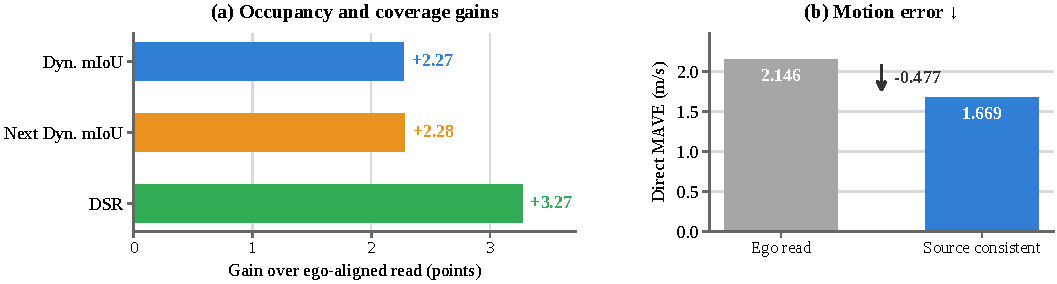
\includegraphics[width=\textwidth]{Fig8-address-benefit.pdf}
  \caption{Measured advantage of source-consistent address construction over
  ego-aligned reading. Values are derived from the matched controlled settings
  in Table~\ref{tab:supp_address_rule}.}
  \label{fig:supp_address_profile}
\end{figure}

\section{Implementation and Scope}
\label{sec:visuals}

The production configuration uses four cameras, a ResNet-50 backbone, three
decoder stages, a $0.4$ m voxel grid, and a $0.5$ s sampling interval. Models are
optimized with AdamW for 24 epochs. Controlled variants share the same
initialization policy, optimizer, schedule, scene-boundary queue reset, and
InfraOcc evaluator. Only the designated factor is changed.

P/T/R operates on semantic voxel support, matching the InfraOcc label space.
Nearby same-class objects can share support within the local radius; when
history has no supported source, Refresh uses the current-frame feature. The
route target therefore encodes semantic evidence admissibility rather than
instance identity. We report dynamic IoU, Direct MAVE, and DSR jointly so that
semantic recovery, motion error, and support coverage remain visible beyond the
GT-conditioned route diagnostic.
